\documentclass[]{article}
\usepackage{lmodern}
\usepackage{amssymb,amsmath}
\usepackage{ifxetex,ifluatex}
\usepackage{fixltx2e} % provides \textsubscript
\ifnum 0\ifxetex 1\fi\ifluatex 1\fi=0 % if pdftex
  \usepackage[T1]{fontenc}
  \usepackage[utf8]{inputenc}
\else % if luatex or xelatex
  \ifxetex
    \usepackage{mathspec}
  \else
    \usepackage{fontspec}
  \fi
  \defaultfontfeatures{Ligatures=TeX,Scale=MatchLowercase}
\fi
% use upquote if available, for straight quotes in verbatim environments
\IfFileExists{upquote.sty}{\usepackage{upquote}}{}
% use microtype if available
\IfFileExists{microtype.sty}{%
\usepackage[]{microtype}
\UseMicrotypeSet[protrusion]{basicmath} % disable protrusion for tt fonts
}{}
\PassOptionsToPackage{hyphens}{url} % url is loaded by hyperref
\usepackage[unicode=true]{hyperref}
\hypersetup{
            pdftitle={MPSoC-NTM (T-DNC/NTM-MPSoC)},
            pdfauthor={QueenField},
            pdfborder={0 0 0},
            breaklinks=true}
\urlstyle{same}  % don't use monospace font for urls
\usepackage[left = 3cm, right = 2cm, top = 3cm, bottom = 2cm]{geometry}
\usepackage{longtable,booktabs}
% Fix footnotes in tables (requires footnote package)
\IfFileExists{footnote.sty}{\usepackage{footnote}\makesavenoteenv{long table}}{}
\usepackage{graphicx,grffile}
\makeatletter
\def\maxwidth{\ifdim\Gin@nat@width>\linewidth\linewidth\else\Gin@nat@width\fi}
\def\maxheight{\ifdim\Gin@nat@height>\textheight\textheight\else\Gin@nat@height\fi}
\makeatother
% Scale images if necessary, so that they will not overflow the page
% margins by default, and it is still possible to overwrite the defaults
% using explicit options in \includegraphics[width, height, ...]{}
\setkeys{Gin}{width=\maxwidth,height=\maxheight,keepaspectratio}
\IfFileExists{parskip.sty}{%
\usepackage{parskip}
}{% else
\setlength{\parindent}{0pt}
\setlength{\parskip}{6pt plus 2pt minus 1pt}
}
\setlength{\emergencystretch}{3em}  % prevent overfull lines
\providecommand{\tightlist}{%
  \setlength{\itemsep}{0pt}\setlength{\parskip}{0pt}}
\setcounter{secnumdepth}{0}
% Redefines (sub)paragraphs to behave more like sections
\ifx\paragraph\undefined\else
\let\oldparagraph\paragraph
\renewcommand{\paragraph}[1]{\oldparagraph{#1}\mbox{}}
\fi
\ifx\subparagraph\undefined\else
\let\oldsubparagraph\subparagraph
\renewcommand{\subparagraph}[1]{\oldsubparagraph{#1}\mbox{}}
\fi

% set default figure placement to htbp
\makeatletter
\def\fps@figure{htbp}
\makeatother


\title{MPSoC-NTM (T-DNC/NTM-MPSoC)}
\author{QueenField}
\date{}

\begin{document}
\maketitle

\begin{figure}
\centering
\includegraphics{../icon.jpg}
\caption{QueenField}
\end{figure}

\section{0. INTRODUCTION}\label{introduction}

\subsection{0.0. DO-254}\label{do-254}

\subsubsection{0.0.1. HARDWARE PLANNING
PROCESS}\label{hardware-planning-process}

\paragraph{0.0.1.1. Plan for Hardware Aspects of
Certification}\label{plan-for-hardware-aspects-of-certification}

\paragraph{0.0.1.2. Hardware Design Plan}\label{hardware-design-plan}

\paragraph{0.0.1.3. Hardware Validation
Plan}\label{hardware-validation-plan}

\paragraph{0.0.1.4. Hardware Verification
Plan}\label{hardware-verification-plan}

\paragraph{0.0.1.5. Hardware Configuration Management
Plan}\label{hardware-configuration-management-plan}

\paragraph{0.0.1.6. Hardware Process Assurance
Plan}\label{hardware-process-assurance-plan}

\subsubsection{0.0.2. HARDWARE DESIGN
PROCESS}\label{hardware-design-process}

\paragraph{0.0.2.1 Requirements Capture
Process}\label{requirements-capture-process}

\paragraph{0.0.2.2 Conceptual Design
Process}\label{conceptual-design-process}

\paragraph{0.0.2.3 Detailed Design
Process}\label{detailed-design-process}

\paragraph{0.0.2.4 Implementation Process}\label{implementation-process}

\paragraph{0.0.2.5 Production Transition
Process}\label{production-transition-process}

\subsubsection{0.0.3. VALIDATION AND VERIFICATION
PROCESS}\label{validation-and-verification-process}

\paragraph{0.0.3.1 Validation Process}\label{validation-process}

\paragraph{0.0.3.2 Verification Process}\label{verification-process}

\subsubsection{0.0.4. CONFIGURATION MANAGEMENT
PROCESS}\label{configuration-management-process}

\subsubsection{0.0.5. PROCESS ASSURANCE}\label{process-assurance}

\subsubsection{0.0.6. CERTIFICATION LIAISON
PROCESS}\label{certification-liaison-process}

\subsubsection{0.0.7. HARDWARE DESIGN LIFECYCLE
DATA}\label{hardware-design-lifecycle-data}

\paragraph{0.0.7.1 Certification
Authority}\label{certification-authority}

\paragraph{0.0.7.2 Certification Reviews}\label{certification-reviews}

\paragraph{0.0.7.3 Scheduling of Reviews}\label{scheduling-of-reviews}

\subsubsection{0.0.8. ADDITIONAL
CONSIDERATIONS}\label{additional-considerations}

\paragraph{0.0.8.1 Previously Developed
Hardware}\label{previously-developed-hardware}

\paragraph{0.0.8.2 Commercial Components
Usage}\label{commercial-components-usage}

\subsection{0.1. BEST PRACTICES}\label{best-practices}

\subsubsection{0.1.1. HARDWARE}\label{hardware}

\subsubsection{0.1.2. SOFTWARE}\label{software}

\section{1. METHODOLOGY}\label{methodology}

\begin{figure}
\centering
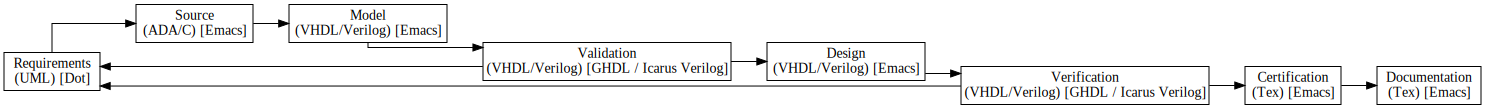
\includegraphics{../doc/project.png}
\caption{Project Workflow}
\end{figure}

\subsection{1.1. Requirements}\label{requirements}

\begin{figure}
\centering
\includegraphics{../requirements/uml_diagrams_overview.png}
\caption{UML Diagrams Overview}
\end{figure}

\subsubsection{1.1.1. Structural UML
diagrams}\label{structural-uml-diagrams}

\paragraph{1.1.1.1. Class diagram}\label{class-diagram}

\paragraph{1.1.1.2. Component diagram}\label{component-diagram}

\paragraph{1.1.1.3. Composite diagram}\label{composite-diagram}

\paragraph{1.1.1.4. Deployment diagram}\label{deployment-diagram}

\paragraph{1.1.1.5. Object diagram}\label{object-diagram}

\paragraph{1.1.1.6. Package diagram}\label{package-diagram}

\paragraph{1.1.1.7. Profile diagram}\label{profile-diagram}

\subsubsection{1.1.2. Behavioral UML
diagrams}\label{behavioral-uml-diagrams}

\paragraph{1.1.2.1. Activity diagram}\label{activity-diagram}

\paragraph{1.1.2.2. Communication diagram}\label{communication-diagram}

\paragraph{1.1.2.3. Interaction diagram}\label{interaction-diagram}

\paragraph{1.1.2.4. Sequence diagram}\label{sequence-diagram}

\paragraph{1.1.2.5. State diagram}\label{state-diagram}

\paragraph{1.1.2.6. Timing diagram}\label{timing-diagram}

\paragraph{1.1.2.7. Use diagram}\label{use-diagram}

\subsection{1.2. Source}\label{source}

\subsubsection{1.2.1. Ada Language}\label{ada-language}

\subsubsection{1.2.2. C Language}\label{c-language}

\subsection{1.3. Model}\label{model}

\subsubsection{1.3.1. VHDL}\label{vhdl}

\subsubsection{1.3.2. Verilog}\label{verilog}

\subsection{1.5. Validation}\label{validation}

\subsubsection{1.5.1. VHDL}\label{vhdl-1}

\subsubsection{1.5.2. Verilog}\label{verilog-1}

\subsection{1.5. Design}\label{design}

\subsubsection{1.5.1. VHDL}\label{vhdl-2}

\subsubsection{1.5.2. Verilog}\label{verilog-2}

\subsection{1.6. Verification}\label{verification}

\subsubsection{1.6.1. OSVVM-VHDL}\label{osvvm-vhdl}

\paragraph{1.6.1.1. OSVVM Checker}\label{osvvm-checker}

\paragraph{1.6.1.2. OSVVM Stimulus}\label{osvvm-stimulus}

\paragraph{1.6.1.3. OSVVM Testbench}\label{osvvm-testbench}

\subsubsection{1.6.2. UVM-Verilog}\label{uvm-verilog}

\begin{figure}
\centering
\includegraphics{../bench/uvm-testbench.png}
\caption{UVM Diagram Overview}
\end{figure}

\paragraph{1.6.2.1. UVM Agent}\label{uvm-agent}

\paragraph{1.6.2.2. UVM Driver}\label{uvm-driver}

\paragraph{1.6.2.3. UVM Enviroment}\label{uvm-enviroment}

\paragraph{1.6.2.4. UVM Monitor}\label{uvm-monitor}

\paragraph{1.6.2.5. UVM Scoreboard}\label{uvm-scoreboard}

\paragraph{1.6.2.6. UVM Sequence}\label{uvm-sequence}

\paragraph{1.6.2.7. UVM Sequencer}\label{uvm-sequencer}

\paragraph{1.6.2.8. UVM Subscriber}\label{uvm-subscriber}

\paragraph{1.6.2.9. UVM Test}\label{uvm-test}

\paragraph{1.6.2.10. UVM Testbench}\label{uvm-testbench}

\paragraph{1.6.2.11. UVM Transaction}\label{uvm-transaction}

\section{2. PROJECTS}\label{projects}

\subsection{2.1. INTERFACE}\label{interface}

\subsubsection{2.1.1. INSTRUCTION CACHE}\label{instruction-cache}

\paragraph{2.1.1.1 Instruction INPUTS/OUTPUTS AMBA4 AXI-Lite
Bus}\label{instruction-inputsoutputs-amba4-axi-lite-bus}

\subparagraph{2.1.1.1.1. Signals of the Read and Write Address
channels}\label{signals-of-the-read-and-write-address-channels}

\begin{longtable}[]{@{}lllll@{}}
\toprule
Write Port & Read Port & Size & Direction & Description\tabularnewline
\midrule
\endhead
\texttt{AWID} & \texttt{ARID} & \texttt{AXI\_ID\_WIDTH} & Output &
Address ID, to identify multiple streams\tabularnewline
\texttt{AWADDR} & \texttt{ARADDR} & \texttt{AXI\_ADDR\_WIDTH} & Output &
Address of the first beat of the burst\tabularnewline
\texttt{AWLEN} & \texttt{ARLEN} & 8 & Output & Number of beats inside
the burst\tabularnewline
\texttt{AWSIZE} & \texttt{ARSIZE} & 3 & Output & Size of each
beat\tabularnewline
\texttt{AWBURST} & \texttt{ARBURST} & 2 & Output & Type of the
burst\tabularnewline
\texttt{AWLOCK} & \texttt{ARLOCK} & 1 & Output & Lock type, to provide
atomic operations\tabularnewline
\texttt{AWCACHE} & \texttt{ARCACHE} & 4 & Output & Memory type, progress
through the system\tabularnewline
\texttt{AWPROT} & \texttt{ARPROT} & 3 & Output & Protection
type\tabularnewline
\texttt{AWQOS} & \texttt{ARQOS} & 4 & Output & Quality of Service of the
transaction\tabularnewline
\texttt{AWREGION} & \texttt{ARREGION} & 4 & Output & Region identifier,
physical to logical\tabularnewline
\texttt{AWUSER} & \texttt{ARUSER} & \texttt{AXI\_USER\_WIDTH} & Output &
User-defined data\tabularnewline
\texttt{AWVALID} & \texttt{ARVALID} & 1 & Output & xVALID handshake
signal\tabularnewline
\texttt{AWREADY} & \texttt{ARREADY} & 1 & Input & xREADY handshake
signal\tabularnewline
\bottomrule
\end{longtable}

\subparagraph{2.1.1.1.2. Signals of the Read and Write Data
channels}\label{signals-of-the-read-and-write-data-channels}

\begin{longtable}[]{@{}lllll@{}}
\toprule
Write Port & Read Port & Size & Direction & Description\tabularnewline
\midrule
\endhead
\texttt{WID} & \texttt{RID} & \texttt{AXI\_ID\_WIDTH} & Output & Data
ID, to identify multiple streams\tabularnewline
\texttt{WDATA} & \texttt{RDATA} & \texttt{AXI\_DATA\_WIDTH} & Output &
Read/Write data\tabularnewline
\texttt{-\/-} & \texttt{RRESP} & 2 & Output & Read response, current
RDATA status\tabularnewline
\texttt{WSTRB} & \texttt{-\/-} & \texttt{AXI\_STRB\_WIDTH} & Output &
Byte strobe, WDATA signal\tabularnewline
\texttt{WLAST} & \texttt{RLAST} & 1 & Output & Last beat
identifier\tabularnewline
\texttt{WUSER} & \texttt{RUSER} & \texttt{AXI\_USER\_WIDTH} & Output &
User-defined data\tabularnewline
\texttt{WVALID} & \texttt{RVALID} & 1 & Output & xVALID handshake
signal\tabularnewline
\texttt{WREADY} & \texttt{RREADY} & 1 & Input & xREADY handshake
signal\tabularnewline
\bottomrule
\end{longtable}

\subparagraph{2.1.1.1.3. Signals of the Write Response
channel}\label{signals-of-the-write-response-channel}

\begin{longtable}[]{@{}llll@{}}
\toprule
Write Port & Size & Direction & Description\tabularnewline
\midrule
\endhead
\texttt{BID} & \texttt{AXI\_ID\_WIDTH} & Input & Write response ID, to
identify multiple streams\tabularnewline
\texttt{BRESP} & 2 & Input & Write response, to specify the burst
status\tabularnewline
\texttt{BUSER} & \texttt{AXI\_USER\_WIDTH} & Input & User-defined
data\tabularnewline
\texttt{BVALID} & 1 & Input & xVALID handshake signal\tabularnewline
\texttt{BREADY} & 1 & Output & xREADY handshake signal\tabularnewline
\bottomrule
\end{longtable}

\paragraph{2.1.1.2. Instruction INPUTS/OUTPUTS AMBA3 AHB-Lite
Bus}\label{instruction-inputsoutputs-amba3-ahb-lite-bus}

\begin{longtable}[]{@{}llll@{}}
\toprule
Port & Size & Direction & Description\tabularnewline
\midrule
\endhead
\texttt{HRESETn} & 1 & Input & Asynchronous Active Low
Reset\tabularnewline
\texttt{HCLK} & 1 & Input & System Clock Input\tabularnewline
& & &\tabularnewline
\texttt{IHSEL} & 1 & Output & Instruction Bus Select\tabularnewline
\texttt{IHADDR} & \texttt{PLEN} & Output & Instruction Address
Bus\tabularnewline
\texttt{IHRDATA} & \texttt{XLEN} & Input & Instruction Read Data
Bus\tabularnewline
\texttt{IHWDATA} & \texttt{XLEN} & Output & Instruction Write Data
Bus\tabularnewline
\texttt{IHWRITE} & 1 & Output & Instruction Write Select\tabularnewline
\texttt{IHSIZE} & 3 & Output & Instruction Transfer Size\tabularnewline
\texttt{IHBURST} & 3 & Output & Instruction Transfer Burst
Size\tabularnewline
\texttt{IHPROT} & 4 & Output & Instruction Transfer Protection
Level\tabularnewline
\texttt{IHTRANS} & 2 & Output & Instruction Transfer Type\tabularnewline
\texttt{IHMASTLOCK} & 1 & Output & Instruction Transfer Master
Lock\tabularnewline
\texttt{IHREADY} & 1 & Input & Instruction Slave Ready
Indicator\tabularnewline
\texttt{IHRESP} & 1 & Input & Instruction Transfer
Response\tabularnewline
\bottomrule
\end{longtable}

\paragraph{2.1.1.3. Instruction INPUTS/OUTPUTS Wishbone
Bus}\label{instruction-inputsoutputs-wishbone-bus}

\begin{longtable}[]{@{}llll@{}}
\toprule
Port & Size & Direction & Description\tabularnewline
\midrule
\endhead
\texttt{rst} & 1 & Input & Synchronous Active High Reset\tabularnewline
\texttt{clk} & 1 & Input & System Clock Input\tabularnewline
& & &\tabularnewline
\texttt{iadr} & \texttt{AW} & Input & Instruction Address
Bus\tabularnewline
\texttt{idati} & \texttt{DW} & Input & Instruction Input
Bus\tabularnewline
\texttt{idato} & \texttt{DW} & Output & Instruction Output
Bus\tabularnewline
\texttt{isel} & \texttt{DW/8} & Input & Byte Select
Signals\tabularnewline
\texttt{iwe} & 1 & Input & Write Enable Input\tabularnewline
\texttt{istb} & 1 & Input & Strobe Signal/Core Select
Input\tabularnewline
\texttt{icyc} & 1 & Input & Valid Bus Cycle Input\tabularnewline
\texttt{iack} & 1 & Output & Bus Cycle Acknowledge Output\tabularnewline
\texttt{ierr} & 1 & Output & Bus Cycle Error Output\tabularnewline
\texttt{iint} & 1 & Output & Interrupt Signal Output\tabularnewline
\bottomrule
\end{longtable}

\subsubsection{2.1.2. DATA CACHE}\label{data-cache}

\paragraph{2.1.2.1. Data INPUTS/OUTPUTS AMBA4 AXI-Lite
Bus}\label{data-inputsoutputs-amba4-axi-lite-bus}

\subparagraph{2.1.2.1.1. Signals of the Read and Write Address
channels}\label{signals-of-the-read-and-write-address-channels-1}

\begin{longtable}[]{@{}lllll@{}}
\toprule
Write Port & Read Port & Size & Direction & Description\tabularnewline
\midrule
\endhead
\texttt{AWID} & \texttt{ARID} & \texttt{AXI\_ID\_WIDTH} & Output &
Address ID, to identify multiple streams\tabularnewline
\texttt{AWADDR} & \texttt{ARADDR} & \texttt{AXI\_ADDR\_WIDTH} & Output &
Address of the first beat of the burst\tabularnewline
\texttt{AWLEN} & \texttt{ARLEN} & 8 & Output & Number of beats inside
the burst\tabularnewline
\texttt{AWSIZE} & \texttt{ARSIZE} & 3 & Output & Size of each
beat\tabularnewline
\texttt{AWBURST} & \texttt{ARBURST} & 2 & Output & Type of the
burst\tabularnewline
\texttt{AWLOCK} & \texttt{ARLOCK} & 1 & Output & Lock type, to provide
atomic operations\tabularnewline
\texttt{AWCACHE} & \texttt{ARCACHE} & 4 & Output & Memory type, progress
through the system\tabularnewline
\texttt{AWPROT} & \texttt{ARPROT} & 3 & Output & Protection
type\tabularnewline
\texttt{AWQOS} & \texttt{ARQOS} & 4 & Output & Quality of Service of the
transaction\tabularnewline
\texttt{AWREGION} & \texttt{ARREGION} & 4 & Output & Region identifier,
physical to logical\tabularnewline
\texttt{AWUSER} & \texttt{ARUSER} & \texttt{AXI\_USER\_WIDTH} & Output &
User-defined data\tabularnewline
\texttt{AWVALID} & \texttt{ARVALID} & 1 & Output & xVALID handshake
signal\tabularnewline
\texttt{AWREADY} & \texttt{ARREADY} & 1 & Input & xREADY handshake
signal\tabularnewline
\bottomrule
\end{longtable}

\subparagraph{2.1.2.1.2. Signals of the Read and Write Data
channels}\label{signals-of-the-read-and-write-data-channels-1}

\begin{longtable}[]{@{}lllll@{}}
\toprule
Write Port & Read Port & Size & Direction & Description\tabularnewline
\midrule
\endhead
\texttt{WID} & \texttt{RID} & \texttt{AXI\_ID\_WIDTH} & Output & Data
ID, to identify multiple streams\tabularnewline
\texttt{WDATA} & \texttt{RDATA} & \texttt{AXI\_DATA\_WIDTH} & Output &
Read/Write data\tabularnewline
\texttt{-\/-} & \texttt{RRESP} & 2 & Output & Read response, current
RDATA status\tabularnewline
\texttt{WSTRB} & \texttt{-\/-} & \texttt{AXI\_STRB\_WIDTH} & Output &
Byte strobe, WDATA signal\tabularnewline
\texttt{WLAST} & \texttt{RLAST} & 1 & Output & Last beat
identifier\tabularnewline
\texttt{WUSER} & \texttt{RUSER} & \texttt{AXI\_USER\_WIDTH} & Output &
User-defined data\tabularnewline
\texttt{WVALID} & \texttt{RVALID} & 1 & Output & xVALID handshake
signal\tabularnewline
\texttt{WREADY} & \texttt{RREADY} & 1 & Input & xREADY handshake
signal\tabularnewline
\bottomrule
\end{longtable}

\subparagraph{2.1.2.1.3. Signals of the Write Response
channel}\label{signals-of-the-write-response-channel-1}

\begin{longtable}[]{@{}llll@{}}
\toprule
Write Port & Size & Direction & Description\tabularnewline
\midrule
\endhead
\texttt{BID} & \texttt{AXI\_ID\_WIDTH} & Input & Write response ID, to
identify multiple streams\tabularnewline
\texttt{BRESP} & 2 & Input & Write response, to specify the burst
status\tabularnewline
\texttt{BUSER} & \texttt{AXI\_USER\_WIDTH} & Input & User-defined
data\tabularnewline
\texttt{BVALID} & 1 & Input & xVALID handshake signal\tabularnewline
\texttt{BREADY} & 1 & Output & xREADY handshake signal\tabularnewline
\bottomrule
\end{longtable}

\paragraph{2.1.2.2. Data INPUTS/OUTPUTS AMBA3 AHB-Lite
Bus}\label{data-inputsoutputs-amba3-ahb-lite-bus}

\begin{longtable}[]{@{}llll@{}}
\toprule
Port & Size & Direction & Description\tabularnewline
\midrule
\endhead
\texttt{HRESETn} & 1 & Input & Asynchronous Active Low
Reset\tabularnewline
\texttt{HCLK} & 1 & Input & System Clock Input\tabularnewline
& & &\tabularnewline
\texttt{DHSEL} & 1 & Output & Data Bus Select\tabularnewline
\texttt{DHADDR} & \texttt{PLEN} & Output & Data Address
Bus\tabularnewline
\texttt{DHRDATA} & \texttt{XLEN} & Input & Data Read Data
Bus\tabularnewline
\texttt{DHWDATA} & \texttt{XLEN} & Output & Data Write Data
Bus\tabularnewline
\texttt{DHWRITE} & 1 & Output & Data Write Select\tabularnewline
\texttt{DHSIZE} & 3 & Output & Data Transfer Size\tabularnewline
\texttt{DHBURST} & 3 & Output & Data Transfer Burst Size\tabularnewline
\texttt{DHPROT} & 4 & Output & Data Transfer Protection
Level\tabularnewline
\texttt{DHTRANS} & 2 & Output & Data Transfer Type\tabularnewline
\texttt{DHMASTLOCK} & 1 & Output & Data Transfer Master
Lock\tabularnewline
\texttt{DHREADY} & 1 & Input & Data Slave Ready Indicator\tabularnewline
\texttt{DHRESP} & 1 & Input & Data Transfer Response\tabularnewline
\bottomrule
\end{longtable}

\paragraph{2.1.2.3. Data INPUTS/OUTPUTS Wishbone
Bus}\label{data-inputsoutputs-wishbone-bus}

\begin{longtable}[]{@{}llll@{}}
\toprule
Port & Size & Direction & Description\tabularnewline
\midrule
\endhead
\texttt{rst} & 1 & Input & Synchronous Active High Reset\tabularnewline
\texttt{clk} & 1 & Input & System Clock Input\tabularnewline
& & &\tabularnewline
\texttt{dadr} & \texttt{AW} & Input & Data Address Bus\tabularnewline
\texttt{ddati} & \texttt{DW} & Input & Data Input Bus\tabularnewline
\texttt{ddato} & \texttt{DW} & Output & Data Output Bus\tabularnewline
\texttt{dsel} & \texttt{DW/8} & Input & Byte Select
Signals\tabularnewline
\texttt{dwe} & 1 & Input & Write Enable Input\tabularnewline
\texttt{dstb} & 1 & Input & Strobe Signal/Core Select
Input\tabularnewline
\texttt{dcyc} & 1 & Input & Valid Bus Cycle Input\tabularnewline
\texttt{dack} & 1 & Output & Bus Cycle Acknowledge Output\tabularnewline
\texttt{derr} & 1 & Output & Bus Cycle Error Output\tabularnewline
\texttt{dint} & 1 & Output & Interrupt Signal Output\tabularnewline
\bottomrule
\end{longtable}

\subsection{2.2. FUNCTIONALITY}\label{functionality}

\subsubsection{2.2.1. Structure}\label{structure}

\subsubsection{2.2.2. Behavior}\label{behavior}

\subsection{2.3. REGISTERS}\label{registers}

\subsection{2.4. INTERRUPTIONS}\label{interruptions}

\section{3. ORGANIZATION}\label{organization}

\subsection{3.1. Mechanics}\label{mechanics}

\subsection{3.2. Information}\label{information}

\subsubsection{3.2.1. Bit}\label{bit}

\subsubsection{3.2.2. Logic Gate}\label{logic-gate}

\paragraph{3.2.2.1. YES/NOT Gate}\label{yesnot-gate}

\paragraph{3.2.2.2. AND/NAND Gate}\label{andnand-gate}

\paragraph{3.2.2.3. OR/NOR Gate}\label{ornor-gate}

\paragraph{3.2.2.4. XOR/XNOR Gate}\label{xorxnor-gate}

\subsubsection{3.2.3. Combinational Logic}\label{combinational-logic}

\paragraph{3.2.3.1. Arithmetic Circuits}\label{arithmetic-circuits}

\paragraph{3.2.3.2. Logic Circuits}\label{logic-circuits}

\subsubsection{3.2.4. Finite State Machine}\label{finite-state-machine}

\subsubsection{3.2.5. Pushdown Automaton}\label{pushdown-automaton}

\subsection{3.3. Neural Network}\label{neural-network}

\subsubsection{3.3.1. Feedforward Neural
Network}\label{feedforward-neural-network}

\subsubsection{3.3.2. Long Short Term Memory Neural
Network}\label{long-short-term-memory-neural-network}

\subsubsection{3.3.3. Transformer Neural
Network}\label{transformer-neural-network}

\subsection{3.4. Turing Machine}\label{turing-machine}

\subsubsection{3.4.1. Neural Turing
Machine}\label{neural-turing-machine}

\paragraph{3.4.1.1. Feedforward Neural Turing
Machine}\label{feedforward-neural-turing-machine}

\paragraph{3.4.1.2. LSTM Neural Turing
Machine}\label{lstm-neural-turing-machine}

\paragraph{3.4.1.3. Transformer Neural Turing
Machine}\label{transformer-neural-turing-machine}

\subsubsection{3.4.2. Differentiable Neural
Computer}\label{differentiable-neural-computer}

\paragraph{3.4.2.1. Feedforward Differentiable Neural
Computer}\label{feedforward-differentiable-neural-computer}

\paragraph{3.4.2.2. LSTM Differentiable Neural
Computer}\label{lstm-differentiable-neural-computer}

\paragraph{3.4.2.3. Transformer Differentiable Neural
Computer}\label{transformer-differentiable-neural-computer}

\subsection{3.5. Computer Architecture}\label{computer-architecture}

\subsubsection{3.5.1. von Neumann
Architecture}\label{von-neumann-architecture}

\paragraph{3.5.1.1. Control Unit}\label{control-unit}

\paragraph{3.5.1.2. ALU}\label{alu}

\paragraph{3.5.1.3. Memory Unit}\label{memory-unit}

\paragraph{3.5.1.4. I/O Unit}\label{io-unit}

\subsubsection{3.5.2. Harvard Architecture}\label{harvard-architecture}

\paragraph{3.5.2.1. Control Unit}\label{control-unit-1}

\paragraph{3.5.2.2. ALU}\label{alu-1}

\paragraph{3.5.2.3.Memory Unit}\label{memory-unit-1}

\paragraph{3.5.2.4.I/O Unit}\label{io-unit-1}

\subsection{3.6. Advanced Computer
Architecture}\label{advanced-computer-architecture}

\subsubsection{3.6.1. Processing Unit}\label{processing-unit}

\paragraph{3.6.1.1. SISD}\label{sisd}

\paragraph{3.6.1.2. SIMD}\label{simd}

\paragraph{3.6.1.3. MISD}\label{misd}

\paragraph{3.6.1.4. MIMD}\label{mimd}

\subsubsection{3.6.2. System on Chip}\label{system-on-chip}

\paragraph{3.6.2.1. Bus on Chip}\label{bus-on-chip}

\paragraph{3.6.2.2. Network on Chip}\label{network-on-chip}

\subsubsection{3.6.3. Multi Processor System on
Chip}\label{multi-processor-system-on-chip}

\section{4. HARDWARE WORKFLOW}\label{hardware-workflow}

\textbf{1. System Level (SystemC/SystemVerilog)}

The System Level abstraction of a system only looks at its biggest
building blocks like processing units or peripheral devices. At this
level the circuit is usually described using traditional programming
languages like SystemC or SystemVerilog. Sometimes special software
libraries are used that are aimed at simulation circuits on the system
level. The IEEE 1685-2009 standard defines the IP-XACT file format that
can be used to represent designs on the system level and building blocks
that can be used in such system level designs.

\textbf{2. Behavioral \& Register Transfer Level (VHDL/Verilog)}

At the Behavioural Level abstraction a language aimed at hardware
description such as Verilog or VHDL is used to describe the circuit, but
so-called behavioural modeling is used in at least part of the circuit
description. In behavioural modeling there must be a language feature
that allows for imperative programming to be used to describe data paths
and registers. This is the always -block in Verilog and the process
-block in VHDL.

A design in Register Transfer Level representation is usually stored
using HDLs like Verilog and VHDL. But only a very limited subset of
features is used, namely minimalistic always blocks (Verilog) or process
blocks (VHDL) that model the register type used and unconditional
assignments for the datapath logic. The use of HDLs on this level
simplifies simulation as no additional tools are required to simulate a
design in Register Transfer Level representation.

\textbf{3. Logical Gate}

At the Logical Gate Level the design is represented by a netlist that
uses only cells from a small number of single-bit cells, such as basic
logic gates (AND, OR, NOT, XOR, etc.) and registers (usually D-Type
Flip-flops). A number of netlist formats exists that can be used on this
level such as the Electronic Design Interchange Format (EDIF), but for
ease of simulation often a HDL netlist is used. The latter is a HDL file
(Verilog or VHDL) that only uses the most basic language constructs for
instantiation and connecting of cells.

\textbf{4. Physical Gate}

On the Physical Gate Level only gates are used that are physically
available on the target architecture. In some cases this may only be
NAND, NOR and NOT gates as well as D-Type registers. In the case of an
FPGA-based design the Physical Gate Level representation is a netlist of
LUTs with optional output registers, as these are the basic building
blocks of FPGA logic cells.

\textbf{5. Switch Level}

A Switch Level representation of a circuit is a netlist utilizing single
transistors as cells. Switch Level modeling is possible in Verilog and
VHDL, but is seldom used in modern designs, as in modern digital ASIC or
FPGA flows the physical gates are considered the atomic build blocks of
the logic circuit.

\begin{enumerate}
\def\labelenumi{\arabic{enumi}.}
\item
  Settings → Apps → Apps \& features → Related settings, Programs and
  Features → Turn Windows features on or off → Windows Subsystem for
  Linux
\item
  Microsoft Store → INSTALL UBUNTU
\end{enumerate}

Front-End and Back-End Library type:

\begin{verbatim}
sudo apt update
sudo apt upgrade

sudo apt install bison cmake flex freeglut3-dev libcairo2-dev libgsl-dev \
libncurses-dev libx11-dev m4 python-tk python3-tk swig tcl tcl-dev tk-dev tcsh
\end{verbatim}

Synthesizer Library type:

\begin{verbatim}
sudo apt update
sudo apt upgrade
\end{verbatim}

\begin{verbatim}
sudo apt -y install build-essential clang bison flex \
libreadline-dev gawk tcl-dev libffi-dev git make gnat \
graphviz xdot pkg-config python3 libboost-system-dev \
libboost-python-dev libboost-filesystem-dev zlib1g-dev
\end{verbatim}

\subsection{4.1. FRONT-END OPEN SOURCE
TOOLS}\label{front-end-open-source-tools}

\begin{figure}
\centering
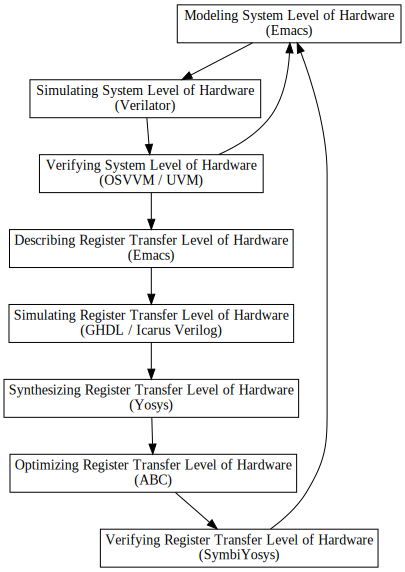
\includegraphics{../doc/front-end.png}
\caption{Front-End}
\end{figure}

\subsubsection{4.1.1. Modeling System Level of
Hardware}\label{modeling-system-level-of-hardware}

\emph{A System Description Language Editor is a computer tool that
allows to generate software code. A System Description Language is a
formal language, which comprises a Programming Language (input),
producing a Hardware Description (output). Programming languages are
used in computer programming to implement algorithms. The description of
a programming language is split into the two components of syntax (form)
and semantics (meaning).}

\textbf{System Description Language Editor}

type:

\begin{verbatim}
git clone https://github.com/emacs-mirror/emacs
\end{verbatim}

\subsubsection{4.1.2. Simulating System Level of
Hardware}\label{simulating-system-level-of-hardware}

\emph{A System Description Language Simulator (translator) is a computer
program that translates computer code written in a Programming Language
(the source language) into a Hardware Description Language (the target
language). The compiler is primarily used for programs that translate
source code from a high-level programming language to a low-level
language to create an executable program.}

\textbf{SystemVerilog System Description Language Simulator}

type:

\begin{verbatim}
git clone http://git.veripool.org/git/verilator

cd verilator
autoconf
./configure
make
sudo make install
\end{verbatim}

\begin{verbatim}
cd sim/verilog/regression/wb/vtor
source SIMULATE-IT
\end{verbatim}

\begin{verbatim}
cd sim/verilog/regression/ahb3/vtor
source SIMULATE-IT
\end{verbatim}

\begin{verbatim}
cd sim/verilog/regression/axi4/vtor
source SIMULATE-IT
\end{verbatim}

\subsubsection{4.1.3. Verifying System Level of
Hardware}\label{verifying-system-level-of-hardware}

\emph{A UVM standard improves interoperability and reduces the cost of
repurchasing and rewriting IP for each new project or Electronic Design
Automation tool. It also makes it easier to reuse verification
components. The UVM Class Library provides generic utilities, such as
component hierarchy, Transaction Library Model or configuration
database, which enable the user to create virtually any structure wanted
for the testbench.}

\textbf{SystemVerilog System Description Language Verifier}

type:

\begin{verbatim}
git clone https://github.com/QueenField/UVM
\end{verbatim}

\subsubsection{4.1.4. Describing Register Transfer Level of
Hardware}\label{describing-register-transfer-level-of-hardware}

\emph{A Hardware Description Language Editor is any editor that allows
to generate hardware code. Hardware Description Language is a
specialized computer language used to describe the structure and
behavior of digital logic circuits. It allows for the synthesis of a HDL
into a netlist, which can then be synthesized, placed and routed to
produce the set of masks used to create an integrated circuit.}

\textbf{Hardware Description Language Editor}

type:

\begin{verbatim}
git clone https://github.com/emacs-mirror/emacs
\end{verbatim}

\subsubsection{4.1.5. Simulating Register Transfer Level of
Hardware}\label{simulating-register-transfer-level-of-hardware}

\emph{A Hardware Description Language Simulator uses mathematical models
to replicate the behavior of an actual hardware device. Simulation
software allows for modeling of circuit operation and is an invaluable
analysis tool. Simulating a circuit's behavior before actually building
it can greatly improve design efficiency by making faulty designs known
as such, and providing insight into the behavior of electronics circuit
designs.}

\textbf{VHDL Hardware Description Language Simulator}

type:

\begin{verbatim}
git clone https://github.com/ghdl/ghdl

cd ghdl
./configure --prefix=/usr/local
make
sudo make install
\end{verbatim}

\begin{verbatim}
cd sim/vhdl/regression/wb/ghdl
source SIMULATE-IT
\end{verbatim}

\begin{verbatim}
cd sim/vhdl/regression/ahb3/ghdl
source SIMULATE-IT
\end{verbatim}

\begin{verbatim}
cd sim/vhdl/regression/axi4/ghdl
source SIMULATE-IT
\end{verbatim}

\textbf{Verilog Hardware Description Language Simulator}

type:

\begin{verbatim}
git clone https://github.com/steveicarus/iverilog

cd iverilog
sh autoconf.sh
./configure
make
sudo make install
\end{verbatim}

\begin{verbatim}
cd sim/verilog/regression/wb/iverilog
source SIMULATE-IT
\end{verbatim}

\begin{verbatim}
cd sim/verilog/regression/ahb3/iverilog
source SIMULATE-IT
\end{verbatim}

\begin{verbatim}
cd sim/verilog/regression/axi4/iverilog
source SIMULATE-IT
\end{verbatim}

\subsubsection{4.1.6. Synthesizing Register Transfer Level of
Hardware}\label{synthesizing-register-transfer-level-of-hardware}

\emph{A Hardware Description Language Synthesizer turns a RTL
implementation into a Logical Gate Level implementation. Logical design
is a step in the standard design cycle in which the functional design of
an electronic circuit is converted into the representation which
captures logic operations, arithmetic operations, control flow, etc. In
EDA parts of the logical design is automated using synthesis tools based
on the behavioral description of the circuit.}

\textbf{Verilog Hardware Description Language Synthesizer}

type:

\begin{verbatim}
git clone https://github.com/YosysHQ/yosys

cd yosys
make
sudo make install
\end{verbatim}

\begin{verbatim}
cd synthesis/yosys
source SYNTHESIZE-IT
\end{verbatim}

\textbf{VHDL Hardware Description Language Synthesizer}

type for Plugin:

\begin{verbatim}
git clone https://github.com/ghdl/ghdl-yosys-plugin

cd ghdl-yosys-plugin
make GHDL=/usr/local
sudo yosys-config --exec mkdir -p --datdir/plugins
sudo yosys-config --exec cp "ghdl.so" --datdir/plugins/ghdl.so
\end{verbatim}

\begin{verbatim}
cd synthesis/yosys
source SYNTHESIZE-IT
\end{verbatim}

\subsubsection{4.1.7. Optimizing Register Transfer Level of
Hardware}\label{optimizing-register-transfer-level-of-hardware}

\emph{A Hardware Description Language Optimizer finds an equivalent
representation of the specified logic circuit under specified
constraints (minimum area, pre-specified delay). This tool combines
scalable logic optimization based on And-Inverter Graphs (AIGs),
optimal-delay DAG-based technology mapping for look-up tables and
standard cells, and innovative algorithms for sequential synthesis and
verification.}

\textbf{Verilog Hardware Description Language Optimizer}

type:

\begin{verbatim}
git clone https://github.com/YosysHQ/yosys

cd yosys
make
sudo make install
\end{verbatim}

\begin{verbatim}
cd synthesis/yosys
source SYNTHESIZE-IT
\end{verbatim}

\subsubsection{4.1.8. Verifying Register Transfer Level of
Hardware}\label{verifying-register-transfer-level-of-hardware}

\emph{A Hardware Description Language Verifier proves or disproves the
correctness of intended algorithms underlying a hardware system with
respect to a certain formal specification or property, using formal
methods of mathematics. Formal verification uses modern techniques
(SAT/SMT solvers, BDDs, etc.) to prove correctness by essentially doing
an exhaustive search through the entire possible input space (formal
proof).}

\textbf{Verilog Hardware Description Language Verifier}

type:

\begin{verbatim}
git clone https://github.com/YosysHQ/SymbiYosys
\end{verbatim}

\subsection{4.2. BACK-END OPEN SOURCE
TOOLS}\label{back-end-open-source-tools}

\begin{figure}
\centering
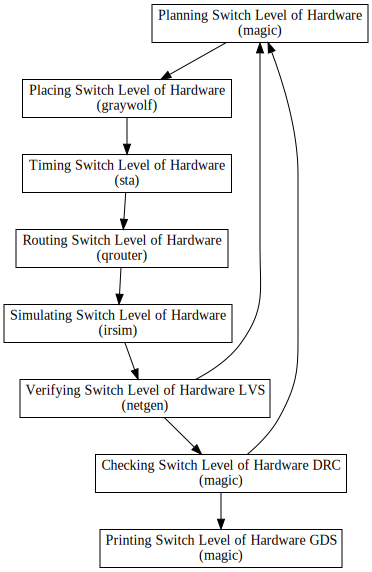
\includegraphics{../doc/back-end.png}
\caption{Back-End}
\end{figure}

\textbf{Library}

type:

\begin{verbatim}
sudo apt update
sudo apt upgrade

sudo apt install bison cmake flex freeglut3-dev libcairo2-dev libgsl-dev \
libncurses-dev libx11-dev m4 python-tk python3-tk swig tcl tcl-dev tk-dev tcsh
\end{verbatim}

\textbf{Back-End Workflow Qflow}

type:

\begin{verbatim}
git clone https://github.com/RTimothyEdwards/qflow

cd qflow
./configure
make
sudo make install
\end{verbatim}

\begin{verbatim}
mkdir qflow
cd qflow
\end{verbatim}

\subsubsection{4.2.1. Planning Switch Level of
Hardware}\label{planning-switch-level-of-hardware}

\emph{A Floor-Planner of an Integrated Circuit (IC) is a schematic
representation of tentative placement of its major functional blocks. In
modern electronic design process floor-plans are created during the
floor-planning design stage, an early stage in the hierarchical approach
to Integrated Circuit design. Depending on the design methodology being
followed, the actual definition of a floor-plan may differ.}

\textbf{Floor-Planner}

type:

\begin{verbatim}
git clone https://github.com/RTimothyEdwards/magic

cd magic
./configure
make
sudo make install
\end{verbatim}

\subsubsection{4.2.2. Placing Switch Level of
Hardware}\label{placing-switch-level-of-hardware}

\emph{A Standard Cell Placer takes a given synthesized circuit netlist
together with a technology library and produces a valid placement
layout. The layout is optimized according to the aforementioned
objectives and ready for cell resizing and buffering, a step essential
for timing and signal integrity satisfaction. Physical design flow are
iterated a number of times until design closure is achieved.}

\textbf{Standard Cell Placer}

type:

\begin{verbatim}
git clone https://github.com/rubund/graywolf

cd graywolf
mkdir build
cd build
cmake ..
make
sudo make install
\end{verbatim}

\subsubsection{4.2.3. Timing Switch Level of
Hardware}\label{timing-switch-level-of-hardware}

\emph{A Standard Cell Timing-Analizer is a simulation method of
computing the expected timing of a digital circuit without requiring a
simulation of the full circuit. High-performance integrated circuits
have traditionally been characterized by the clock frequency at which
they operate. Measuring the ability of a circuit to operate at the
specified speed requires an ability to measure, during the design
process, its delay at numerous steps.}

\textbf{Standard Cell Timing-Analizer}

type:

\begin{verbatim}
git clone https://github.com/The-OpenROAD-Project/OpenSTA

cd OpenSTA
mkdir build
cd build
cmake ..
make
sudo make install
\end{verbatim}

\subsubsection{4.2.4. Routing Switch Level of
Hardware}\label{routing-switch-level-of-hardware}

\emph{A Standard Cell Router takes pre-existing polygons consisting of
pins on cells, and pre-existing wiring called pre-routes. Each of these
polygons are associated with a net. The primary task of the router is to
create geometries such that all terminals assigned to the same net are
connected, no terminals assigned to different nets are connected, and
all design rules are obeyed.}

\textbf{Standard Cell Router}

type:

\begin{verbatim}
git clone https://github.com/RTimothyEdwards/qrouter

cd qrouter
./configure
make
sudo make install
\end{verbatim}

\subsubsection{4.2.5. Simulating Switch Level of
Hardware}\label{simulating-switch-level-of-hardware}

\emph{A Standard Cell Simulator treats transistors as ideal switches.
Extracted capacitance and lumped resistance values are used to make the
switch a little bit more realistic than the ideal, using the RC time
constants to predict the relative timing of events. This simulator
represents a circuit in terms of its exact transistor structure but
describes the electrical behavior in a highly idealized way.}

\textbf{Standard Cell Simulator}

type:

\begin{verbatim}
git clone https://github.com/RTimothyEdwards/irsim

cd irsim
./configure
make
sudo make install
\end{verbatim}

\subsubsection{4.2.6. Verifying Switch Level of Hardware
LVS}\label{verifying-switch-level-of-hardware-lvs}

\emph{A Standard Cell Verifier compares netlists, a process known as LVS
(Layout vs.~Schematic). This step ensures that the geometry that has
been laid out matches the expected circuit. The greatest need for LVS is
in large analog or mixed-signal circuits that cannot be simulated in
reasonable time. LVS can be done faster than simulation, and provides
feedback that makes it easier to find errors.}

\textbf{Standard Cell Verifier}

type:

\begin{verbatim}
git clone https://github.com/RTimothyEdwards/netgen

cd netgen
./configure
make
sudo make install
\end{verbatim}

\begin{verbatim}
cd synthesis/qflow
source FLOW-IT
\end{verbatim}

\subsubsection{4.2.7. Checking Switch Level of Hardware
DRC}\label{checking-switch-level-of-hardware-drc}

\emph{A Standard Cell Checker is a geometric constraint imposed on
Printed Circuit Board (PCB) and Integrated Circuit (IC) designers to
ensure their designs function properly, reliably, and can be produced
with acceptable yield. Design Rules for production are developed by
hardware engineers based on the capability of their processes to realize
design intent. Design Rule Checking (DRC) is used to ensure that
designers do not violate design rules.}

\textbf{Standard Cell Checker}

type:

\begin{verbatim}
git clone https://github.com/RTimothyEdwards/magic

cd magic
./configure
make
sudo make install
\end{verbatim}

\subsubsection{4.2.8. Printing Switch Level of Hardware
GDS}\label{printing-switch-level-of-hardware-gds}

\emph{A Standard Cell Editor allows to print a set of standard cells.
The standard cell methodology is an abstraction, whereby a low-level
VLSI layout is encapsulated into a logical representation. A standard
cell is a group of transistor and interconnect structures that provides
a boolean logic function (AND, OR, XOR, XNOR, inverters) or a storage
function (flipflop or latch).}

\textbf{Standard Cell Editor}

type:

\begin{verbatim}
git clone https://github.com/RTimothyEdwards/magic

cd magic
./configure
make
sudo make install
\end{verbatim}

\section{5. SOFTWARE WORKFLOW}\label{software-workflow}

\subsection{5.1. BACK-END OPEN SOURCE
TOOLS}\label{back-end-open-source-tools-1}

type:

\begin{verbatim}
sudo apt install autoconf automake autotools-dev curl python3 libmpc-dev \
libmpfr-dev libgmp-dev gawk build-essential bison flex texinfo gperf \
libtool patchutils bc zlib1g-dev libexpat-dev
\end{verbatim}

\subsubsection{5.1.1. MSP430}\label{msp430}

\paragraph{5.1.1.1. MSP430 GNU C/C++}\label{msp430-gnu-cc}

\paragraph{5.1.1.2. MSP430 GNU Go}\label{msp430-gnu-go}

\subsubsection{5.1.2. OpenRISC}\label{openrisc}

\paragraph{5.1.2.1. OpenRISC GNU C/C++}\label{openrisc-gnu-cc}

\paragraph{5.1.2.2. OpenRISC GNU Go}\label{openrisc-gnu-go}

\subsubsection{5.1.3. RISC-V}\label{risc-v}

\paragraph{5.1.3.1. RISC-V GNU C/C++}\label{risc-v-gnu-cc}

type:

\begin{verbatim}
git clone --recursive https://github.com/riscv/riscv-gnu-toolchain

cd riscv-gnu-toolchain

./configure --prefix=/opt/riscv-elf-gcc
sudo make clean
sudo make

./configure --prefix=/opt/riscv-elf-gcc
sudo make clean
sudo make linux

./configure --prefix=/opt/riscv-elf-gcc --enable-multilib
sudo make clean
sudo make linux
\end{verbatim}

\paragraph{5.1.3.2. RISC-V GNU Go}\label{risc-v-gnu-go}

type:

\begin{verbatim}
git clone --recursive https://go.googlesource.com/go riscv-go
cd riscv-go/src
./all.bash
cd ../..
sudo mv riscv-go /opt
\end{verbatim}

\subsection{5.2. FRONT-END OPEN SOURCE
TOOLS}\label{front-end-open-source-tools-1}

\subsubsection{5.2.1. MSP430}\label{msp430-1}

\subsubsection{5.2.2. OpenRISC}\label{openrisc-1}

\subsubsection{5.2.3. RISC-V}\label{risc-v-1}

type:

\begin{verbatim}
sudo apt install device-tree-compiler libglib2.0-dev libpixman-1-dev pkg-config
\end{verbatim}

\paragraph{5.2.3.1. Spike (For Hardware
Engineers)}\label{spike-for-hardware-engineers}

\textbf{Building Proxy Kernel}

type:

\begin{verbatim}
export PATH=/opt/riscv-elf-gcc/bin:${PATH}

git clone --recursive https://github.com/riscv/riscv-pk

cd riscv-pk
mkdir build
cd build
../configure --prefix=/opt/riscv-elf-gcc --host=riscv64-unknown-elf
make
sudo make install
\end{verbatim}

\textbf{Building Spike}

type:

\begin{verbatim}
export PATH=/opt/riscv-elf-gcc/bin:${PATH}

git clone --recursive https://github.com/riscv/riscv-isa-sim

cd riscv-isa-sim
mkdir build
cd build
../configure --prefix=/opt/riscv-elf-gcc
make
sudo make install
\end{verbatim}

\paragraph{5.2.3.2. QEMU (For Software
Engineers)}\label{qemu-for-software-engineers}

type:

\begin{verbatim}
export PATH=/opt/riscv-elf-gcc/bin:${PATH}

git clone --recursive https://github.com/qemu/qemu

cd qemu
./configure --prefix=/opt/riscv-elf-gcc \
--target-list=riscv64-softmmu,riscv32-softmmu,riscv64-linux-user,riscv32-linux-user
make
sudo make install
\end{verbatim}

\end{document}
